% This is a comment.
% the region directly below this comment, up till the command \begin{document} is known as the 'preamble'
% basic setup
\documentclass[12pt]{article}
\usepackage[english]{babel}
\usepackage[utf8]{inputenc}

% for mathematics
\usepackage{amsmath}
\usepackage{amsthm}
% define theorems, lemmas, etc
\newtheorem{theorem}{Theorem}
\newtheorem{lemma}{Lemma}
\newtheorem{corollary}{Corollary}
\newtheorem{definition}{Definition}
\newtheorem{example}{Example}
\usepackage{amssymb}

% for adjusting margins
\usepackage{geometry}
\geometry{
	a4paper,
 	left=26mm,
 	right=20mm,
 	top=33mm,
 	bottom=38mm
}

\usepackage{array}
\usepackage{booktabs}
\setlength{\heavyrulewidth}{1.5pt}
\setlength{\abovetopsep}{4pt}

% for introducing urls
\usepackage{url}

% for colored text
\usepackage{color}

% for creating lists
\usepackage{enumerate}

% change font to times new roman
\usepackage{times}

% include algorithm package
\usepackage[]{algorithm2e}

% include bbm package to support indicator variable
\usepackage{bbm}

% include picture
\usepackage{graphicx}

% include bibliography
\usepackage[superscript,biblabel]{cite}

%~~~~~~~~~~~~~~~~~~~~~~~~~~~~~~~~~~~~~~~~~~~~~~~~~~~~~~~~~~~~~~~~~~~~~~~~~~~~~~
% the region between \begin{document} ... \end{document} is known as the 'text'
\begin{document}
\begin{titlepage}
	\centering
	\vspace*{.09\textheight}
	{\LARGE\bfseries CS2102 Database\\
Project Report\par}
	\vspace{1.5cm}
	{\huge Carolend\par}
	\vspace{1cm}
	{\scshape\Large Dong Shaocong, He Xinyi, Liu Yulin, Wang Zexin\par}
	\vspace{6cm}
	
	\vspace{3cm}
	{\Large Department of Mathematics\\[3mm]
National University of Singapore\\[3mm]
AY2017/18 Semester 1\par}
\end{titlepage}

\section*{Abstract}
\newpage

\section*{Acknowledge}
We would like to thank Associate Professor Bressan Stephane for his helpful supervision
throughout the course of this project.
\newpage
\tableofcontents
\newpage

\section{Introduction}
In this project, we are required to build a stuff sharing website. the system allows people to borrow or lend stuff that they own (tools, appliances, furniture or books) either free or for a fee. Users advertise stuff available (what stuff, where to pick up and return, when it is available, etc.) or can browse the available stuff and bid to borrow some stuff. The stuff owner or the system (your choice) chooses the successful bid. Each user has an account. Administrators can create, modify and delete all entries.
\subsection{Developing Specifications}

After seeing through the relevant products specifications and the website requirements, we decided to use $PHP$ as back end programming language, $Javascript$ as front end developing language, $MySQL$ as our database. We used $Laravel$, which is the most popular web application framework for $PHP$.\\
\\
From the project requirement, Eloquent ORM in built in Laravel to access and manipulate the database is not allowed. Therefore, anything related to database management, access, and manipulation is down by importing $PHP$ $mysqli$ library and execute raw $SQL$ queries.\\
\\
To develop this web application, we utilise the Model View Controller ($MVC$) framework.\\

\begin{figure}[h]
      \centering
	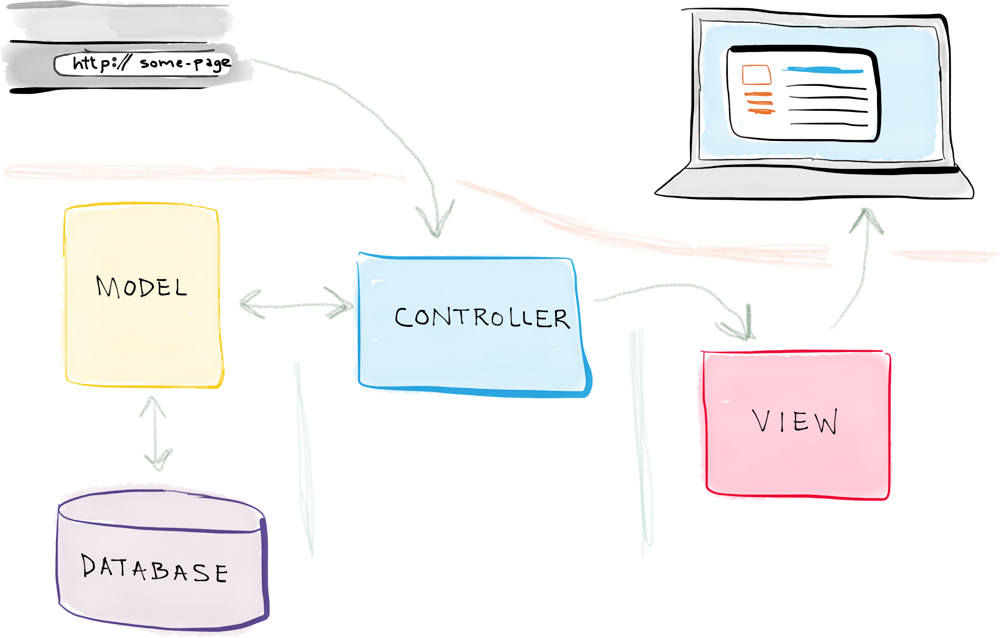
\includegraphics[scale=0.2]{MVC_framework.png}
      \caption{Model View Controller (MVC)}
\end{figure}

We use $CSS$ Scaffolding in Laravel to take care of the views. Buttons and redirections from the user side are implemented in $Javascript$. The models and controllers are written in $PHP$. The specific $MySQL$ database we used it $root$ user's database named $blog$. The website is still hosted on \url{localhost:8000} only.\\
\\
From our modelling for this problem, there are two types of users. The admin users will have different interfaces and unlimited access to all entries. From the user management button in the admin user's profile page. All the users information can be modified and deleted. New users can be added on this panel as well.\\
\\

\newpage

\section{Database Design}

\subsection{Entity-Relationship Diagram}
\newpage

\subsection{Entities}

\begin{center}
\begin{tabular}{|c|c|}
\multicolumn{2}{c}{Users}\\[2mm]
\hline
Attribute & Domain\\
\hline
email & VARCHAR(64)\\
username & VARCHAR(64) \\
password & VARCHAR(64) \\
mobile & INT(8) \\
address & VARCHAR(128) \\
points\_available & INT(3) \\
credit\_rating & NUMERIC \\
created\_at & TIMESTAMP \\
\hline
\end{tabular}
\end{center}



\begin{center}
\begin{tabular}{|c|c|}
\multicolumn{2}{c}{Items}\\[2mm]
\hline
Attribute & Domain\\
\hline
name & VARCHAR(64)\\
avatar & VARCHAR(256) \\
owner & VARCHAR(64) \\
description & TEXT \\
available & VARCHAR(5)\\
created\_at & TIMESTAMP \\
\hline
\end{tabular}
\end{center}

\begin{center}
\begin{tabular}{|c|c|}
\multicolumn{2}{c}{Posts}\\[2mm]
\hline
Attribute & Domain\\
\hline
item & VARCHAR(64)\\
title & VARCHAR(64) \\
location & VARCHAR(128) \\
description & TEXT \\
start & TIMESTAMP \\
end & TIMESTAMP \\
created\_at & TIMESTAMP \\
\hline
\end{tabular}
\end{center}

\begin{center}
\begin{tabular}{|c|c|}
\multicolumn{2}{c}{Bids}\\[2mm]
\hline
Attribute & Domain\\
\hline
bidder & VARCHAR(64)\\
post & VARCHAR(64) \\
status & CHAR(7) \\
points & INT(3) \\
created\_at & TIMESTAMP \\
\hline
\end{tabular}
\end{center}

\begin{center}
\begin{tabular}{|c|c|}
\multicolumn{2}{c}{Loans}\\[2mm]
\hline
Attribute & Domain\\
\hline
bid & VARCHAR(64)\\
post & VARCHAR(64) \\
start & TIMESTAMP \\
end & TIMESTAMP \\
comments & TEXT \\
status & VARCHAR(8) \\
created\_at & TIMESTAMP \\
\hline
\end{tabular}
\end{center}


\subsection{Relational Schema}

\subsection{Schema Functions}

\newpage

\section{SQL Queries}

\subsection{Simple Queries}

\subsection{Aggregate Queries}

\subsection{Nested Queries}

\subsection{Queries using INNER JOIN}

\subsection{Queries using EXISTS}

\subsection{Queries using set operations}

\subsection{Insertions, Deletions and Updates}

\subsection{Stored Procedures and Triggers}

\newpage

\section{Web Interface Design}
We aims to have a friendly, easy-to-use interface for our web application. The following sections are about the pages in our web interface.
\subsection{Sign Up Page}
\begin{figure}[h]
      \centering
	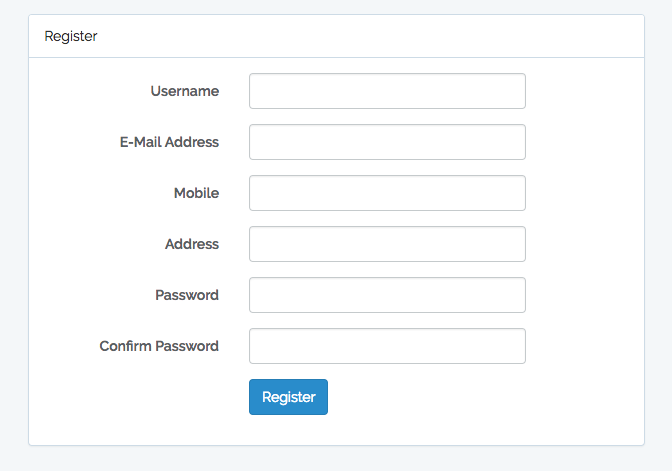
\includegraphics[scale=0.5]{register.png}
      \caption{New User registration page}
\end{figure}
From this page, new users will be able to sign up and enter our system.

\subsection{Log In Page}
Other users will be able to log in via this page.
\begin{figure}[h]
      \centering
	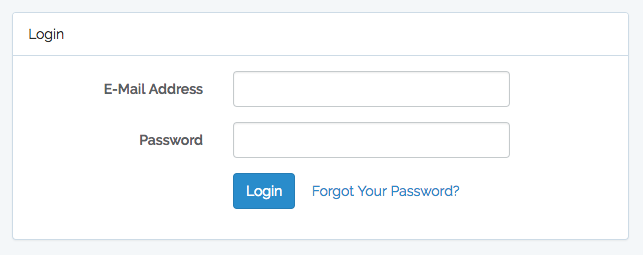
\includegraphics[scale=0.5]{login.png}
      \caption{User login page}
\end{figure}
\newpage

\subsection{Application}
Upon logging in, the user will be directed to his dashboard. He can easily see the points available for him or her. Besides that, the items the user owning, the posts he or she has submitted, the posts the user is currently bidding and the items the user is currently borrowing will be displayed sequentially thought this the page.\\
\begin{figure}[h]
      \centering
	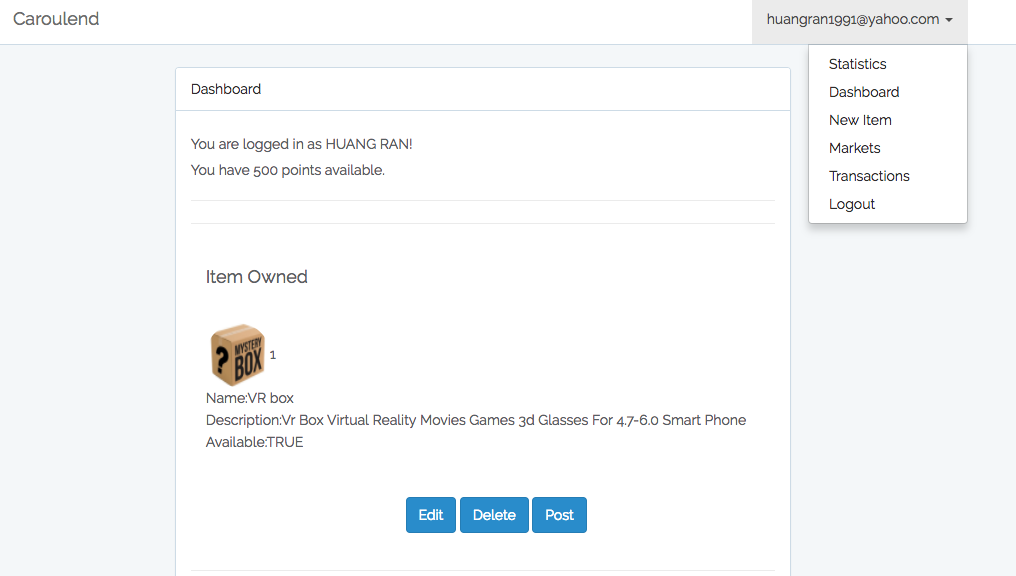
\includegraphics[scale=0.3]{dashboard.png}
      \caption{User login page}
\end{figure}
In addition, from the top right drop down list, the user can go to other pages ranging form his or her using statistics. User can also create new item, go to the posting markets and checkout current transactions and transacting history. This includes the user's posts that are being bid by other users, the user's current lending items and the past transactions.

\subsection{Administration}
There is a special type of user called admin user. They have their admin column equal to 1 and the can have unlimited access to access, delete, update and create any entries in our database. Users are not able to sign up an admin account. The only possible way to become an admin is to update the table in our database directly. Implemented in this way, the administration page is very secure and the current normal users' information are properly protected.
\begin{figure}[h]
      \centering
	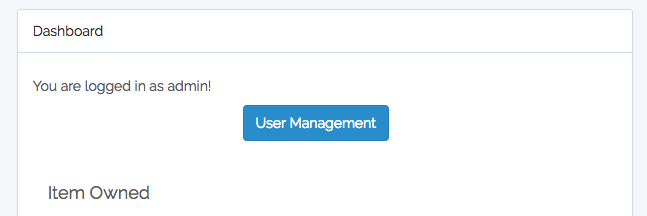
\includegraphics[scale=0.3]{admin.png}
      \caption{User login page}
\end{figure}
As shown in this screen shot, the admin user can access any entries inside this application. If he or she wants to manage the current users, they can do so by clicking the user management button and the user records can be updated, deleted or created on our administration user management panel.

\newpage

\section{Sample table and diagram insertion}
\begin{center}
\begin{tabular}{|c|c|c|c|}
\hline
StrikePrice & Closed-form formula & Ordinary Monte Carlo & Control Variate\\
\hline
105&10.0022021172&10.005252032814727& 10.005252032814751\\
110&8.02638469385&8.0166707887876427& 8.016670788787664\\ 
115&6.37924904693&6.3659464432937911& 6.3659464432937733\\ 
120&5.02541348179&5.0148870431746415& 5.0148870431746184\\
125&3.92690420603&3.9241698581683577& 3.9241698581683728\\
130&3.04592058431&3.044679765401427&  3.0446797654014213\\
135&2.34679877596&2.3310307686205207& 2.3310307686205225\\
140&1.79723400902&1.8055531375480696& 1.8055531375480751\\
145&1.36889248498&1.3630119824610754& 1.3630119824610734\\
150&1.03756650489&1.0254470920297398& 1.0254470920297361\\
155&0.783018613011&0.77819086371547286&0.77819086371547308\\
160&0.588637155719&0.5924848566970754& 0.59248485669707973\\
165&0.440997057228&0.44342591182216823&0.4434259118221664\\
170&0.329392108384&0.32449718396190719&0.32449718396190735\\
175&0.245381782063&0.2462392632801686& 0.24623926328016907\\
180&0.182377553986&0.17995020687354496&0.1799502068735449\\
185&0.13528073067&0.13478417666883458&0.13478417666883413\\
190&0.100175092579&0.099449778570450814&0.099449778570450523\\
195&0.0740722950356&0.074452813719303179&0.074452813719303304\\
200&0.0547050187389&0.051631534936688268&0.051631534936688074\\
\hline
\end{tabular}
\end{center}

\begin{figure}[h]
      \centering
	
\includegraphics[scale=0.45]{DefaultItem.png}
      \caption{Effect of control variate in pricing European call options}
\end{figure}
\newpage

\section{Conclusion}

correct way of citing something: \cite{PythonForFinance}

\newpage
\begin{thebibliography}{9}
\bibitem{PythonForFinance} 
Yves Hilpisch,
\textit{Python for Finance}. 
O'Reilly Media, 2015.
 
\bibitem{VarianceReduction} 
Paul Glasserman,
\textit{Monte Carlo methods in financial engineering}.
Springer, 2010.

\bibitem{FiniteDifference} 
Daniel Duffy,
\textit{Finite difference methods in financial engineering: A partial differential equation approach}.
John Wiley\&Sons, 2006.

\bibitem{ContinuityCorrection} 
Mark Broadie, Paul Glasserman, Steven Kou,
\textit{A Continuity Correction for Discrete Barrier Options}.
Mathematical Finance, 1997.

\end{thebibliography}
\end{document}